\documentclass[11pt]{examdesign}
\usepackage{amsmath}
\usepackage{enumitem}
\usepackage{amsfonts}
\usepackage{pgfplots}
\usepackage{pifont}
\usepackage{graphicx}
\usepackage{fancyhdr}
\usepackage{cancel}
\usepackage{gensymb}
\usepackage[american]{circuitikz}

\SectionFont{\large\sffamily}
\Fullpages
\ContinuousNumbering
\usepackage{ulem}
\ProportionalBlanks{2}


\DefineAnswerWrapper{}{}
\NumberOfVersions{1}
%\IncludeFromFile{foobar.tex}
\examname{\Large{Projectiles}}
\class {\Large Physics}

\def \namedata {Name: \hrulefill\\ 
	Date: \hrulefill \\
	Period: \hrulefill \\
	Primary Peer Reviewer: \hrulefill 
	\\
			\begin{tabular}{| p{1cm} | p{1cm} | p{1 cm} | p{1cm} |}
	\hline
		+1 & 0 & -1 & $\Sigma$ 
		\\
		\hline
		& & & \vspace{.5cm}
		\\ \hline
	
	\end{tabular}
	\\
 \vspace{-.6in}
	
}




\begin{document}




\begin{multiplechoice} [title={Multiple Choice},
	rearrange=no]
	\vspace{0.13in}
\textbf{The following information applies to questions 1-3:} 

A projectile is launched multiple times.  The angle of launch is increased from 0\degree to 90\degree in 5\degree increments.  The following data is collected:
	
	\begin{center}
	

	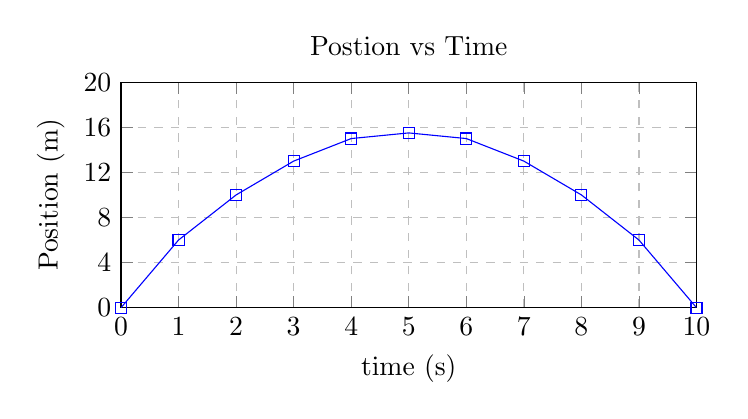
\begin{tikzpicture}
	\begin{axis}[
	title={Postion vs Time},
	xlabel={time (s)},
	ylabel={Position (m)},
	xmin=0, xmax=10,
	ymin=0, ymax=20,
	xtick={0,1,2,3,4,5,6,7,8,9,10},
	ytick={0,4,8,12,16,20},
	ymajorgrids=true,
	xmajorgrids=true,
	grid style=dashed,
	legend pos=south east,
	height=1.75in,
	width=3.5in
	]
	
	\addplot[
	color=blue,
	mark=square,
	]
	coordinates {
		(0,0)(1,6)(2,10)(3,13)(4,15)(5,15.5)(6,15)(7,13)(8,10)(9,6)(10,0)};

	

	
	
	\end{axis}
	\end{tikzpicture}
\end{center}
	\vspace{-0.25in}
	
	\begin{question}
	
At what angle is the range of the projectile greatest?
	 \choice {0\degree}
	 \choice [!]{45\degree}
	 \choice {90\degree}
	 \choice {The range is the same for all angles.}
	\end{question}


\begin{question}
	At what angle was the projectile in the air the longest?
	\choice {0\degree}
	\choice [!]{45\degree}
	\choice {90\degree}
	\choice {The time in the air is the same for all angles.}
\end{question}

\begin{question}
	What two angles result in the same range?
	\choice {30\degree and 40\degree}
	\choice {30\degree and 50\degree}
	\choice {30\degree and 60\degree}
	\choice {30\degree and 70\degree}
\end{question}


	\begin{question}
At the top of its path, a projectile's acceleration is - 
	\choice {0 m/s\textsuperscript{2}}
	\choice {9.81 m/s\textsuperscript{2} downward}
	\choice {9.81 m/s\textsuperscript{2} horizontally}
	\choice {cannot be determined without more information.}
\end{question}

\begin{question}

Two projectiles are launched at the same speed, but different angles.  Their trajectories are shown below: 

	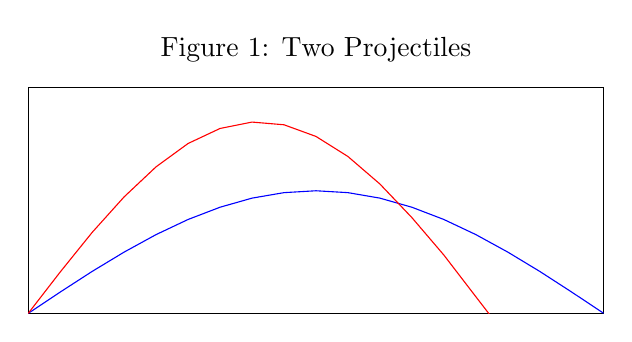
\begin{tikzpicture}
\begin{axis}[
title={Figure 1: Two Projectiles},
xmin=0, xmax=90,
ymin=0, ymax=3,
xtick={-20},
ytick={-20},
ymajorgrids=true,
xmajorgrids=true,
grid style=dashed,
legend pos=south east,
height=1.75in,
width=3.5in
]

\addplot[
color=blue,
mark=none,
]
coordinates {
	(0,0)(5,0.283)(10,0.558)(15,0.815)(20,1.048)(25,1.249)(30,1.412)(35,1.533)(40,1.606)(45,1.631)(50,1.606)(55,1.533)(60,1.412)(65,1.249)(70,1.048)(75,0.815)(80,0.558)(85,0.283)(90,0)};


\addplot[
color=red,
mark=none,
]
coordinates {
	(0,0)(5,0.55)(10,1.077)(15,1.55)(20,1.95)(25,2.26)(30,2.46)(35,2.545)(40,2.509)(45,2.354)(50,2.087)(55,1.721)(60,1.274)(65,0.776)(70,0.222)(75,-0.33)};




\end{axis}
\end{tikzpicture}

If projectile A was launched at a 45 degree angle to the ground, projectile B was launched at an angle - 
\choice{greater than 45\degree}
\choice{less than 45\degree}
\choice{equal to 45\degree}
\choice{there is no way to determine what angle projectile B was launched at.}

	\end{question}



\begin{question}
	
	A projectile's trajectory is shown below: 
	
	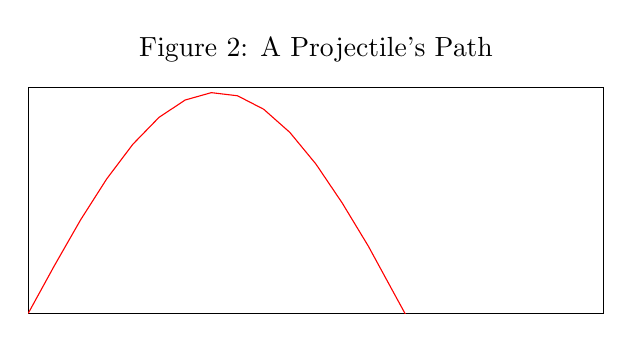
\begin{tikzpicture}
	\begin{axis}[
	title={Figure 2: A Projectile's Path},
	xmin=0, xmax=110,
	ymin=0, ymax=2.6,
	xtick={-20},
	ytick={-20},
	ymajorgrids=true,
	xmajorgrids=true,
	grid style=dashed,
	legend pos=south east,
	height=1.75in,
	width=3.5in
	]
	

	
	
	\addplot[
	color=red,
	mark=none,
	]
	coordinates {
		(0,0)(5,0.55)(10,1.077)(15,1.55)(20,1.95)(25,2.26)(30,2.46)(35,2.545)(40,2.509)(45,2.354)(50,2.087)(55,1.721)(60,1.274)(65,0.776)(70,0.222)(75,-0.33)};
	
	
	
	
	\end{axis}
	\end{tikzpicture}
	
At Point P, the horizontal velocity of the projectile is - 

	\choice{0 m/s}
	\choice{9.81 m/s downward}
	\choice{equal to the initial horizontal velocity.}
	\choice{impossible to determine.}
	
\end{question}
\begin{question}
	
At Point P, the vertical velocity of the projectile is - 

\choice{0 m/s}
\choice{9.81 m/s downward}
\choice{equal to the initial vertical velocity.}
\choice{impossible to determine.}

\end{question}
\end{multiplechoice}

\pagebreak

\begin{shortanswer}[title={Free Response},
	rearrange=no]
	
	\begin{question}
	A projectile is fired from a cannon at a 30-degree angle with the ground and an initial velocity of 100 m/sec. Assuming no air resistance and g=9.81 m/s\textsuperscript{2},	
		\begin{enumerate}
			\item  calculate the time it will spend in the air.
			\vspace{1 in}
			\item Calculate the maximum height of the cannonball.
			\vspace{1 in}
			\item What is the distance the cannonball lands from the cannon?

		\end{enumerate}
		
	\end{question}

\end{shortanswer}
\end{document}


